\documentclass[12pt,a4paper]{report}
\usepackage[utf8]{inputenc}
\usepackage{titlesec}
\usepackage{graphicx}
\usepackage[utf8]{inputenc}
\usepackage[dvipsnames]{xcolor}
\usepackage{color}
\usepackage{imakeidx}
\usepackage[T1]{fontenc}
\usepackage{listings}
\usepackage{fancybox, calc} 
\usepackage{hyperref}
\usepackage{amssymb}
\usepackage{keystroke}
\usepackage{tikz}
\usepackage{geometry}
\geometry{
 a4paper,
 total={170mm,257mm},
 left=20mm,
 top=20mm,
 }


\newtheorem{definition}{Definition} 

\makeindex
\titleformat{\chapter}[hang]{\normalfont\huge\bfseries}{\chaptertitlename\ \thechapter:}{1em}{} 

% Definició dels colors ---------------------------------------------
\definecolor{codegreen}{rgb}{0,0.6,0}
\definecolor{codegray}{rgb}{0.5,0.5,0.5}
\definecolor{codepurple}{rgb}{0.58,0,0.82}
\definecolor{backcolour}{rgb}{0.95,0.95,0.92}

% Definició de l'estil del codi 
\lstdefinestyle{mystyle}{
    backgroundcolor=\color{backcolour},   
    commentstyle=\color{codegreen},
    keywordstyle=\color{magenta},
    numberstyle=\tiny\color{codegray},
    stringstyle=\color{codepurple},
    basicstyle=\footnotesize,
    breakatwhitespace=false,         
    breaklines=true,                 
    captionpos=b,                    
    keepspaces=true,                 
    numbers=left,                    
    numbersep=5pt,                  
    showspaces=false,                
    showstringspaces=false,
    showtabs=false,                  
    tabsize=2
}
\lstset{style=mystyle}


% VARIABLES 
\def \w{$\omega$}
\def \dfa{$FXBP_{DFA} $}
\def \alphabetDFA{$\Sigma$*\dfa}
\def \nfa{$FXBP_{NFA} $}
\def \pfa{$GGR_{PDA} $}
\def \tm{$MSP_{TM} $}
\def \context{$\Phi$}
\def \contextDFA{$\Phi_{DFA}$}
\def \pre{$\Upsilon$}
\def \preDFA{$\Upsilon_{DFA}$}
\def \post{$\Psi$}
\def \postDFA{$\Psi_{DFA}$}
\def \llesca{$\gamma$}


\begin{document}

% Títol de la pràctica -----------------------------------------------
\begin{titlepage}
	\centering
	\includegraphics[width=0.55\textwidth]{udg_logo.png}\par\vspace{1cm}
	{\scshape\LARGE Universitat de girona \par}
	\vspace{1cm}
	{\scshape\Large Pràctica final\par}
	\vspace{1.5cm}
	{\huge\bfseries Fonaments de la computació\par}
	\vspace{2cm}
	{\Large\itshape Francesc Xavier Bullich Parra\par}
	{\Large\itshape Gil Gassó Rovira\par}
	{\Large\itshape Marc Sànchez Pifarré\par}
			
	\vfill
	Tutor de la pràctica\par
	Jaume Rigau

	\vfill

% Bottom of the page
	{\large \today\par}
\end{titlepage}

% Índex -----------------------------------------------
\tableofcontents
\clearpage


\chapter{Introducció}
\setcounter{chapter}{1}

\section{Definicions}

Es defineixen una série de noms que seran utilitzats al llarc de la pràctica per ajudar a la simplificació i l'enteniment de la mateixa. 

\begin{itemize}
\item Definim \dfa{} com l’autòmata finit determinista capaç de reconéixer el llenguatge L(\dfa{}).
\item Definim L (\dfa{}) com el conjunt infinit de mots \w{} que accepta \dfa{}
\item Definim \w{} com un mot tal que \w{} $\in$ L(\dfa{})
\item Definim \alphabetDFA{} com el conjunt de símbols amb el que es construeix el llenguatge L(\dfa{})
\item Definim context \context{} com l’escenari ideal en el que l’autòmata a dissenyar es comportarà de manera correcta, \context{} = < \pre{}, \post{} >  
\item Definim \pre{} com la precondició que s'ha de complir al utilitzar els nostres autòmates. 
\item Definim \post{} com la postcondició de l'autómata.
\end{itemize}

\chapter{Autòmata Finit}

\section{Definició del context}

Sigui \contextDFA{} l'espai de funcionament lògic del nostre autòmata com l'espai estipulat a la Secció 3.Patrons[1]. Per tant acabem d'aquirir totes les definicions assumides a l'enunciat del problema, veure [1].

\textbf{Fem les següents afirmacions sobre \pre{} :}
\begin{itemize}
\item \w{} $\in$ $P_0$ $\wedge$ $P_0$ $\in$ $P$
\item \llesca{} com a llesca continguda dins d'un $P$ on \llesca{} $\in$ \w $\vee$ \llesca{} = $\epsilon$
\end{itemize}

\textbf{Fem les següents afirmacions sobre \post{} :}
\begin{itemize}
\item retorna True quan \dfa{} Accepta \w{} $\leftrightarrow$ $\exists$ \llesca{} $\in$ $P$ que compleix PIP.
\item retorna False quan $\nexists$ \llesca{} $\in$ $P$ que compleix PIP. 
\end{itemize}
on : PIP és la propietat dels patrons implícits parcials definida a [1] apartat 3.3.1. 

\section{Dissenyant el nostre autòmata finit}

Primerament cal observar possibles propietats del problema que ens puguin servir per a la construcció de l’autòmata.

\begin{itemize}
\item Definim 4+ com la seqüència de símbols ‘++++’ d’un mot \w{} comprés dins del llenguatge L(\dfa{}).
\end{itemize}

\textbf{Realitzem les següents observacions :}

\begin{enumerate}
\item Abans i després de la seqüència 4+ hi pot haver qualsevol símbol 0 o més vegades comprés dins de \alphabetDFA{}.
\item Aïllada és la seqüència de simbols ‘-+-’ dins de \w{}
\item Entre dues seqüències 4+ hi trobem 3 aïllades. 
\item 2 aïllades poden compartir el symbol inicial o el symbol final o ambdós. 
\item S’accepta ‘-+-+-’ com a dues cèl·lules aïllades on -+ comparteix - amb +-. 
\item S’accepta ‘-+-+-+-’ coma  tres cèl·lules aïllades on -+ comparteix- amb +-+- i -+-+ comparteix - amb +-.
\item Entre 2 aïllades hi pot aparèixer qualsevol combinació de symbols pertanyent a \alphabetDFA{}.
\item El symbol \Return ens fa tornar a començar a cercar el PIP (RESET). 
\end{enumerate}


Dissenyarem doncs l’autòmata per construcció tenint en compte les anteriors propietats. En la construcció del nostre autòmata reduim el problema al tractament d’un subconjunt dels símbols de l’alfabet, concretament es construeix a partir del subconjunt {+,-}, ja que detectem que el símbol \Return actúa com a RESET. La funció del RESET en \dfa{} és exemplificada al capítol 1 del llibre [1], concretament als exemples 1.15 i 1.17.
 
Incorporarem el RESET al nostre disseny a l’últim pas de la construcció.

\textbf{Fem les següents definicions en l’escenari sense RESET :}

\begin{itemize}
\item Definim pa com la seqüència ‘-+’
\item Definim fa com la seqüència ‘+-’
\item Definim l’operació CONCATENACIÓ amb el symbol | 
\item Definim 3aïllades com :
\begin{itemize}
\item ({+-}* | pa | (-{+-}*)* | pa | (-{+-}*)* | pa | - | {+-}*) $\vee$ ({+-}* | - | fa | (-{+-}*)* | fa | (-{+-}*)* | fa | {+-}*)
\end{itemize}
\end{itemize}

Per tant podem concebre que en un entorn on no hi ha RESET es cerca si el mot conté la següent seqüència de simbols : 

\begin{center}
{+-}* | 4+ | 3aïllades | 4+ | {+-}*
\end{center}

\subsection{Construïm l’autòmata sense RESET}

Veiem que els estats de l'autòmata van avançant a mesura que es van trobant el patró. Hi distingim cicles que ens interessen per controlar els casos que on per exemple hi pot haver qualsevol cosa entre cel·les actives o entre cel·les actives i principi o final del patró. 

\begin{center}
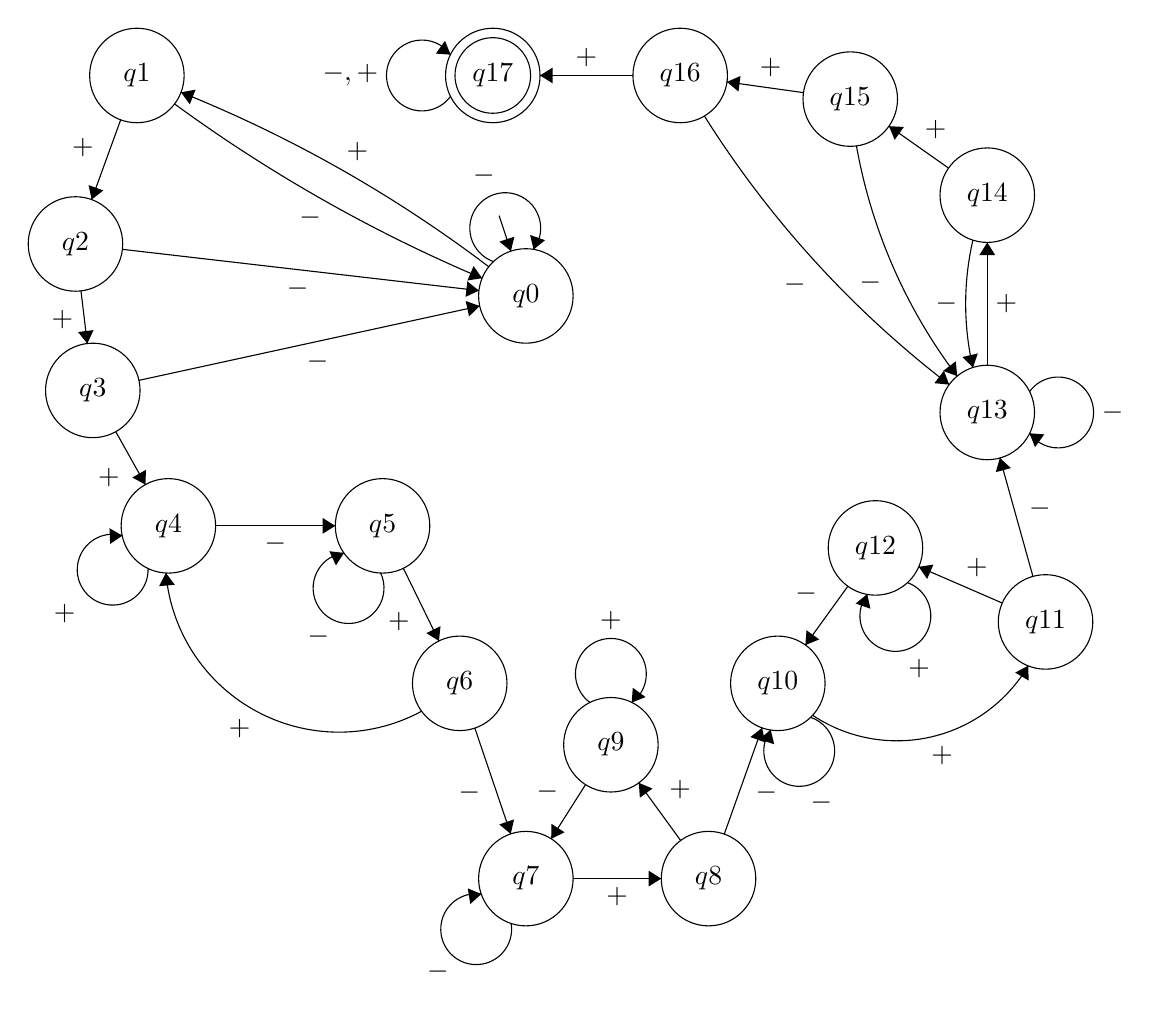
\begin{tikzpicture}[scale=0.2]
\tikzstyle{every node}+=[inner sep=0pt]
\draw [black] (34.2,-17.4) circle (3);
\draw (34.2,-17.4) node {$q0$};
\draw [black] (9.5,-3.4) circle (3);
\draw (9.5,-3.4) node {$q1$};
\draw [black] (5.6,-14.1) circle (3);
\draw (5.6,-14.1) node {$q2$};
\draw [black] (6.7,-23.4) circle (3);
\draw (6.7,-23.4) node {$q3$};
\draw [black] (11.5,-32) circle (3);
\draw (11.5,-32) node {$q4$};
\draw [black] (25.1,-32) circle (3);
\draw (25.1,-32) node {$q5$};
\draw [black] (30,-42) circle (3);
\draw (30,-42) node {$q6$};
\draw [black] (34.2,-54.4) circle (3);
\draw (34.2,-54.4) node {$q7$};
\draw [black] (45.8,-54.4) circle (3);
\draw (45.8,-54.4) node {$q8$};
\draw [black] (39.6,-45.9) circle (3);
\draw (39.6,-45.9) node {$q9$};
\draw [black] (50.2,-42) circle (3);
\draw (50.2,-42) node {$q10$};
\draw [black] (67.2,-38.1) circle (3);
\draw (67.2,-38.1) node {$q11$};
\draw [black] (56.4,-33.4) circle (3);
\draw (56.4,-33.4) node {$q12$};
\draw [black] (63.5,-24.8) circle (3);
\draw (63.5,-24.8) node {$q13$};
\draw [black] (63.5,-11) circle (3);
\draw (63.5,-11) node {$q14$};
\draw [black] (54.8,-4.9) circle (3);
\draw (54.8,-4.9) node {$q15$};
\draw [black] (44,-3.4) circle (3);
\draw (44,-3.4) node {$q16$};
\draw [black] (32.1,-3.4) circle (3);
\draw (32.1,-3.4) node {$q17$};
\draw [black] (32.1,-3.4) circle (2.4);
\draw [black] (12.303,-4.469) arc (68.10472:52.80601:84.368);
\fill [black] (12.3,-4.47) -- (12.86,-5.23) -- (13.23,-4.3);
\draw (23.5,-8.85) node [above] {$+$};
\draw [black] (31.419,-16.275) arc (-112.91179:-126.17748:97.153);
\fill [black] (31.42,-16.27) -- (30.88,-15.5) -- (30.49,-16.42);
\draw (20.5,-11.81) node [below] {$-$};
\draw [black] (8.47,-6.22) -- (6.63,-11.28);
\fill [black] (6.63,-11.28) -- (7.37,-10.7) -- (6.43,-10.36);
\draw (6.79,-7.96) node [left] {$+$};
\draw [black] (5.95,-17.08) -- (6.35,-20.42);
\fill [black] (6.35,-20.42) -- (6.75,-19.57) -- (5.76,-19.69);
\draw (5.49,-18.87) node [left] {$+$};
\draw [black] (8.16,-26.02) -- (10.04,-29.38);
\fill [black] (10.04,-29.38) -- (10.08,-28.44) -- (9.21,-28.93);
\draw (8.44,-28.91) node [left] {$+$};
\draw [black] (8.58,-14.44) -- (31.22,-17.06);
\fill [black] (31.22,-17.06) -- (30.48,-16.47) -- (30.37,-17.46);
\draw (19.7,-16.32) node [below] {$-$};
\draw [black] (9.63,-22.76) -- (31.27,-18.04);
\fill [black] (31.27,-18.04) -- (30.38,-17.72) -- (30.59,-18.7);
\draw (20.97,-20.97) node [below] {$-$};
\draw [black] (32.155,-15.221) arc (250.91269:-37.08731:2.25);
\draw (31.53,-10.4) node [above] {$-$};
\fill [black] (34.69,-14.45) -- (35.42,-13.86) -- (34.47,-13.53);
\draw [black] (14.5,-32) -- (22.1,-32);
\fill [black] (22.1,-32) -- (21.3,-31.5) -- (21.3,-32.5);
\draw (18.3,-32.5) node [below] {$-$};
\draw [black] (26.42,-34.69) -- (28.68,-39.31);
\fill [black] (28.68,-39.31) -- (28.78,-38.37) -- (27.88,-38.81);
\draw (26.85,-38.09) node [left] {$+$};
\draw [black] (24.974,-34.986) arc (25.32189:-262.67811:2.25);
\draw (21.03,-38.42) node [below] {$-$};
\fill [black] (22.65,-33.72) -- (21.72,-33.61) -- (22.14,-34.51);
\draw [black] (27.588,-43.768) arc (-61.55234:-175.2337:11.03);
\fill [black] (11.34,-34.99) -- (10.91,-35.83) -- (11.91,-35.74);
\draw (16.03,-44.28) node [below] {$+$};
\draw [black] (30.96,-44.84) -- (33.24,-51.56);
\fill [black] (33.24,-51.56) -- (33.45,-50.64) -- (32.51,-50.96);
\draw (31.34,-48.92) node [left] {$-$};
\draw [black] (37.2,-54.4) -- (42.8,-54.4);
\fill [black] (42.8,-54.4) -- (42,-53.9) -- (42,-54.9);
\draw (40,-54.9) node [below] {$+$};
\draw [black] (44.03,-51.98) -- (41.37,-48.32);
\fill [black] (41.37,-48.32) -- (41.44,-49.26) -- (42.24,-48.68);
\draw (43.28,-48.77) node [right] {$+$};
\draw [black] (38.277,-43.22) arc (234:-54:2.25);
\draw (39.6,-38.65) node [above] {$+$};
\fill [black] (40.92,-43.22) -- (41.8,-42.87) -- (40.99,-42.28);
\draw [black] (33.264,-57.238) arc (9.47914:-278.52086:2.25);
\draw (28.61,-59.69) node [below] {$-$};
\fill [black] (31.38,-55.38) -- (30.51,-55.02) -- (30.67,-56.01);
\draw [black] (37.99,-48.43) -- (35.81,-51.87);
\fill [black] (35.81,-51.87) -- (36.66,-51.46) -- (35.82,-50.92);
\draw (36.28,-48.85) node [left] {$-$};
\draw [black] (52.27,-44.156) arc (71.56583:-216.43417:2.25);
\draw (52.96,-48.97) node [below] {$-$};
\fill [black] (49.75,-44.95) -- (49.02,-45.55) -- (49.97,-45.87);
\draw [black] (46.8,-51.57) -- (49.2,-44.83);
\fill [black] (49.2,-44.83) -- (48.46,-45.41) -- (49.4,-45.75);
\draw (48.76,-48.96) node [right] {$-$};
\draw [black] (66.103,-40.879) arc (-30.43509:-123.72341:9.668);
\fill [black] (66.1,-40.88) -- (65.27,-41.32) -- (66.13,-41.82);
\draw (60.63,-45.99) node [below] {$+$};
\draw [black] (54.65,-35.83) -- (51.95,-39.57);
\fill [black] (51.95,-39.57) -- (52.83,-39.21) -- (52.02,-38.63);
\draw (52.71,-36.32) node [left] {$-$};
\draw [black] (58.421,-35.601) arc (70.28801:-217.71199:2.25);
\draw (59.17,-40.43) node [below] {$+$};
\fill [black] (55.88,-36.34) -- (55.14,-36.93) -- (56.08,-37.26);
\draw [black] (64.45,-36.9) -- (59.15,-34.6);
\fill [black] (59.15,-34.6) -- (59.68,-35.37) -- (60.08,-34.46);
\draw (62.84,-35.24) node [above] {$+$};
\draw [black] (66.4,-35.21) -- (64.3,-27.69);
\fill [black] (64.3,-27.69) -- (64.04,-28.59) -- (65,-28.33);
\draw (66.12,-30.91) node [right] {$-$};
\draw [black] (66.18,-23.477) arc (144:-144:2.25);
\draw (70.75,-24.8) node [right] {$-$};
\fill [black] (66.18,-26.12) -- (66.53,-27) -- (67.12,-26.19);
\draw [black] (63.5,-21.8) -- (63.5,-14);
\fill [black] (63.5,-14) -- (63,-14.8) -- (64,-14.8);
\draw (64,-17.9) node [right] {$+$};
\draw [black] (61.04,-9.28) -- (57.26,-6.62);
\fill [black] (57.26,-6.62) -- (57.62,-7.49) -- (58.2,-6.67);
\draw (60.22,-7.45) node [above] {$+$};
\draw [black] (51.83,-4.49) -- (46.97,-3.81);
\fill [black] (46.97,-3.81) -- (47.7,-4.42) -- (47.83,-3.43);
\draw (49.75,-3.55) node [above] {$+$};
\draw [black] (41,-3.4) -- (35.1,-3.4);
\fill [black] (35.1,-3.4) -- (35.9,-3.9) -- (35.9,-2.9);
\draw (38.05,-2.9) node [above] {$+$};
\draw [black] (62.587,-21.946) arc (-167.03367:-192.96633:18.031);
\fill [black] (62.59,-21.95) -- (62.9,-21.05) -- (61.92,-21.28);
\draw (61.63,-17.9) node [left] {$-$};
\draw [black] (61.585,-22.492) arc (-142.84995:-169.9215:34.083);
\fill [black] (61.59,-22.49) -- (61.5,-21.55) -- (60.7,-22.16);
\draw (56.79,-16.54) node [left] {$-$};
\draw [black] (61.079,-23.029) arc (-127.49491:-147.82459:65.368);
\fill [black] (61.08,-23.03) -- (60.75,-22.15) -- (60.14,-22.94);
\draw (52.01,-16.65) node [left] {$-$};
\draw [black] (29.42,-4.723) arc (324:36:2.25);
\draw (24.85,-3.4) node [left] {$-,+$};
\fill [black] (29.42,-2.08) -- (29.07,-1.2) -- (28.48,-2.01);
\draw [black] (32.5,-12.3) -- (33.25,-14.55);
\fill [black] (33.25,-14.55) -- (33.47,-13.64) -- (32.52,-13.95);
\draw [black] (10.21,-34.696) arc (2.15723:-285.84277:2.25);
\draw (5.63,-37.59) node [left] {$+$};
\fill [black] (8.58,-32.62) -- (7.76,-32.15) -- (7.8,-33.15);
\end{tikzpicture}
\end{center}

\subsection{Construïm l’Autòmata Complet}

Afegim RESET a l’autòmata, en aquest cas tots els estats menys l’estat final tindran una transició a l’estat inicial amb el símbol \Return. L’estat final com que el mot ja està acceptat tindrà una transició a ell mateix amb el símbol \Return. 


En aquest disseny, per simplificar la codificació del caràcter \Return el codifiquem com una \textit{i}. 
\begin{center}
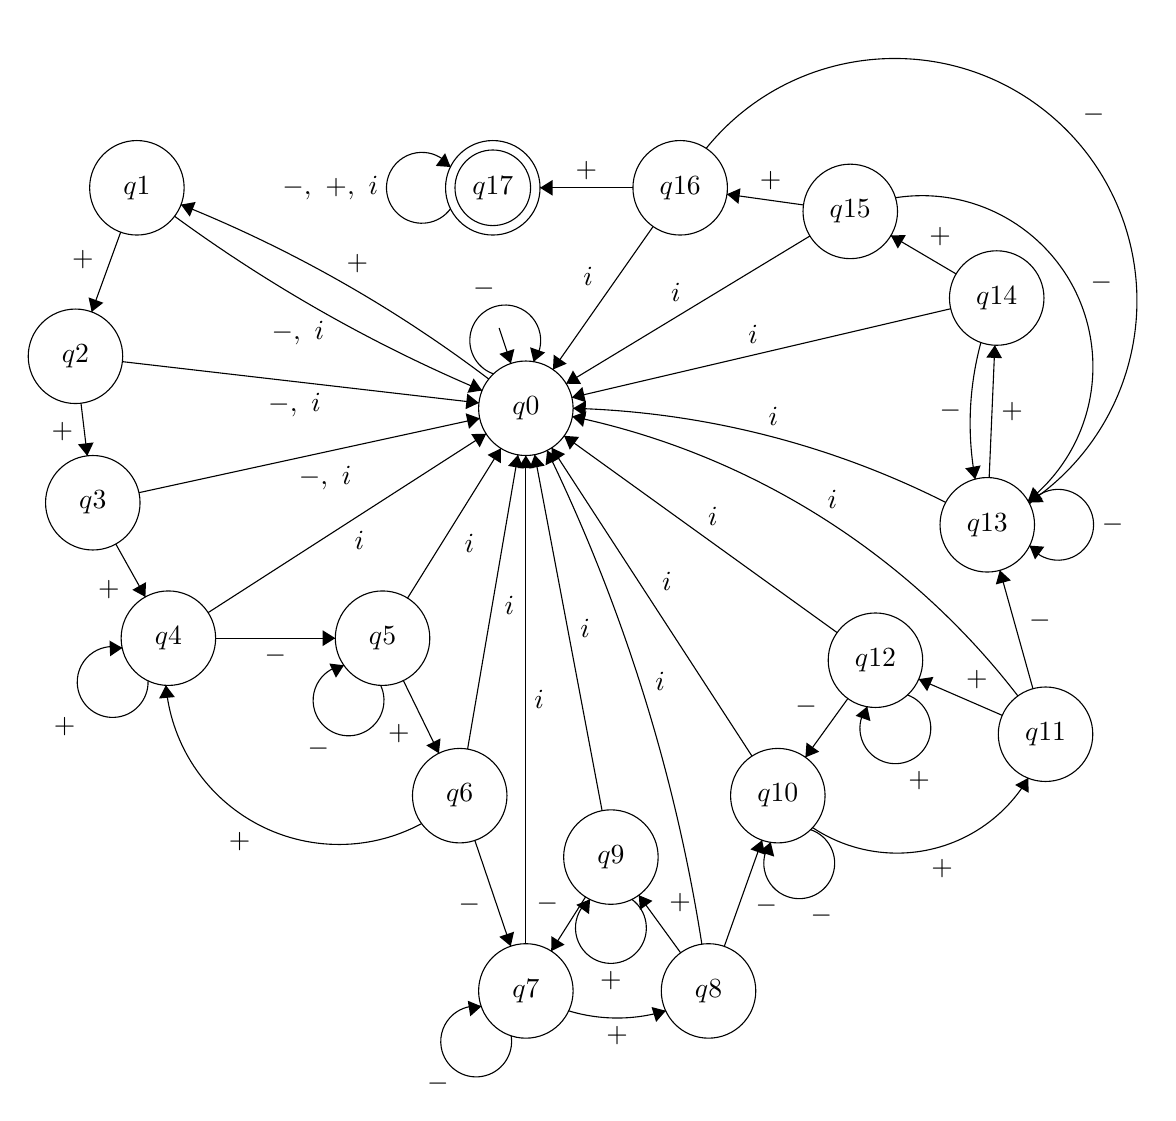
\begin{tikzpicture}[scale=0.2]
\tikzstyle{every node}+=[inner sep=0pt]
\draw [black] (34.2,-17.4) circle (3);
\draw (34.2,-17.4) node {$q0$};
\draw [black] (9.5,-3.4) circle (3);
\draw (9.5,-3.4) node {$q1$};
\draw [black] (5.6,-14.1) circle (3);
\draw (5.6,-14.1) node {$q2$};
\draw [black] (6.7,-23.4) circle (3);
\draw (6.7,-23.4) node {$q3$};
\draw [black] (11.5,-32) circle (3);
\draw (11.5,-32) node {$q4$};
\draw [black] (25.1,-32) circle (3);
\draw (25.1,-32) node {$q5$};
\draw [black] (30,-42) circle (3);
\draw (30,-42) node {$q6$};
\draw [black] (34.2,-54.4) circle (3);
\draw (34.2,-54.4) node {$q7$};
\draw [black] (45.8,-54.4) circle (3);
\draw (45.8,-54.4) node {$q8$};
\draw [black] (39.6,-45.9) circle (3);
\draw (39.6,-45.9) node {$q9$};
\draw [black] (50.2,-42) circle (3);
\draw (50.2,-42) node {$q10$};
\draw [black] (67.2,-38.1) circle (3);
\draw (67.2,-38.1) node {$q11$};
\draw [black] (56.4,-33.4) circle (3);
\draw (56.4,-33.4) node {$q12$};
\draw [black] (63.5,-24.8) circle (3);
\draw (63.5,-24.8) node {$q13$};
\draw [black] (64.1,-10.4) circle (3);
\draw (64.1,-10.4) node {$q14$};
\draw [black] (54.8,-4.9) circle (3);
\draw (54.8,-4.9) node {$q15$};
\draw [black] (44,-3.4) circle (3);
\draw (44,-3.4) node {$q16$};
\draw [black] (32.1,-3.4) circle (3);
\draw (32.1,-3.4) node {$q17$};
\draw [black] (32.1,-3.4) circle (2.4);
\draw [black] (12.303,-4.469) arc (68.10472:52.80601:84.368);
\fill [black] (12.3,-4.47) -- (12.86,-5.23) -- (13.23,-4.3);
\draw (23.5,-8.85) node [above] {$+$};
\draw [black] (31.419,-16.275) arc (-112.91179:-126.17748:97.153);
\fill [black] (31.42,-16.27) -- (30.88,-15.5) -- (30.49,-16.42);
\draw (19.73,-11.81) node [below] {$-,\mbox{ }i$};
\draw [black] (8.47,-6.22) -- (6.63,-11.28);
\fill [black] (6.63,-11.28) -- (7.37,-10.7) -- (6.43,-10.36);
\draw (6.79,-7.96) node [left] {$+$};
\draw [black] (5.95,-17.08) -- (6.35,-20.42);
\fill [black] (6.35,-20.42) -- (6.75,-19.57) -- (5.76,-19.69);
\draw (5.49,-18.87) node [left] {$+$};
\draw [black] (8.16,-26.02) -- (10.04,-29.38);
\fill [black] (10.04,-29.38) -- (10.08,-28.44) -- (9.21,-28.93);
\draw (8.44,-28.91) node [left] {$+$};
\draw [black] (8.58,-14.44) -- (31.22,-17.06);
\fill [black] (31.22,-17.06) -- (30.48,-16.47) -- (30.37,-17.46);
\draw (19.51,-16.39) node [below] {$-,\mbox{ }i$};
\draw [black] (9.63,-22.76) -- (31.27,-18.04);
\fill [black] (31.27,-18.04) -- (30.38,-17.72) -- (30.59,-18.7);
\draw (21.45,-21.03) node [below] {$-,\mbox{ }i$};
\draw [black] (32.155,-15.221) arc (250.91269:-37.08731:2.25);
\draw (31.53,-10.4) node [above] {$-$};
\fill [black] (34.69,-14.45) -- (35.42,-13.86) -- (34.47,-13.53);
\draw [black] (14.5,-32) -- (22.1,-32);
\fill [black] (22.1,-32) -- (21.3,-31.5) -- (21.3,-32.5);
\draw (18.3,-32.5) node [below] {$-$};
\draw [black] (26.42,-34.69) -- (28.68,-39.31);
\fill [black] (28.68,-39.31) -- (28.78,-38.37) -- (27.88,-38.81);
\draw (26.85,-38.09) node [left] {$+$};
\draw [black] (24.974,-34.986) arc (25.32189:-262.67811:2.25);
\draw (21.03,-38.42) node [below] {$-$};
\fill [black] (22.65,-33.72) -- (21.72,-33.61) -- (22.14,-34.51);
\draw [black] (27.588,-43.768) arc (-61.55234:-175.2337:11.03);
\fill [black] (11.34,-34.99) -- (10.91,-35.83) -- (11.91,-35.74);
\draw (16.03,-44.28) node [below] {$+$};
\draw [black] (30.96,-44.84) -- (33.24,-51.56);
\fill [black] (33.24,-51.56) -- (33.45,-50.64) -- (32.51,-50.96);
\draw (31.34,-48.92) node [left] {$-$};
\draw [black] (43.089,-55.662) arc (-73.11558:-106.88442:10.637);
\fill [black] (43.09,-55.66) -- (42.18,-55.42) -- (42.47,-56.37);
\draw (40,-56.62) node [below] {$+$};
\draw [black] (44.03,-51.98) -- (41.37,-48.32);
\fill [black] (41.37,-48.32) -- (41.44,-49.26) -- (42.24,-48.68);
\draw (43.28,-48.77) node [right] {$+$};
\draw [black] (40.923,-48.58) arc (54:-234:2.25);
\draw (39.6,-53.15) node [below] {$+$};
\fill [black] (38.28,-48.58) -- (37.4,-48.93) -- (38.21,-49.52);
\draw [black] (33.264,-57.238) arc (9.47914:-278.52086:2.25);
\draw (28.61,-59.69) node [below] {$-$};
\fill [black] (31.38,-55.38) -- (30.51,-55.02) -- (30.67,-56.01);
\draw [black] (37.99,-48.43) -- (35.81,-51.87);
\fill [black] (35.81,-51.87) -- (36.66,-51.46) -- (35.82,-50.92);
\draw (36.28,-48.85) node [left] {$-$};
\draw [black] (52.27,-44.156) arc (71.56583:-216.43417:2.25);
\draw (52.96,-48.97) node [below] {$-$};
\fill [black] (49.75,-44.95) -- (49.02,-45.55) -- (49.97,-45.87);
\draw [black] (46.8,-51.57) -- (49.2,-44.83);
\fill [black] (49.2,-44.83) -- (48.46,-45.41) -- (49.4,-45.75);
\draw (48.76,-48.96) node [right] {$-$};
\draw [black] (66.103,-40.879) arc (-30.43509:-123.72341:9.668);
\fill [black] (66.1,-40.88) -- (65.27,-41.32) -- (66.13,-41.82);
\draw (60.63,-45.99) node [below] {$+$};
\draw [black] (54.65,-35.83) -- (51.95,-39.57);
\fill [black] (51.95,-39.57) -- (52.83,-39.21) -- (52.02,-38.63);
\draw (52.71,-36.32) node [left] {$-$};
\draw [black] (58.421,-35.601) arc (70.28801:-217.71199:2.25);
\draw (59.17,-40.43) node [below] {$+$};
\fill [black] (55.88,-36.34) -- (55.14,-36.93) -- (56.08,-37.26);
\draw [black] (64.45,-36.9) -- (59.15,-34.6);
\fill [black] (59.15,-34.6) -- (59.68,-35.37) -- (60.08,-34.46);
\draw (62.84,-35.24) node [above] {$+$};
\draw [black] (66.4,-35.21) -- (64.3,-27.69);
\fill [black] (64.3,-27.69) -- (64.04,-28.59) -- (65,-28.33);
\draw (66.12,-30.91) node [right] {$-$};
\draw [black] (66.18,-23.477) arc (144:-144:2.25);
\draw (70.75,-24.8) node [right] {$-$};
\fill [black] (66.18,-26.12) -- (66.53,-27) -- (67.12,-26.19);
\draw [black] (63.62,-21.8) -- (63.98,-13.4);
\fill [black] (63.98,-13.4) -- (63.44,-14.18) -- (64.44,-14.22);
\draw (64.36,-17.62) node [right] {$+$};
\draw [black] (61.52,-8.87) -- (57.38,-6.43);
\fill [black] (57.38,-6.43) -- (57.82,-7.26) -- (58.33,-6.4);
\draw (60.51,-7.15) node [above] {$+$};
\draw [black] (51.83,-4.49) -- (46.97,-3.81);
\fill [black] (46.97,-3.81) -- (47.7,-4.42) -- (47.83,-3.43);
\draw (49.75,-3.55) node [above] {$+$};
\draw [black] (41,-3.4) -- (35.1,-3.4);
\fill [black] (35.1,-3.4) -- (35.9,-3.9) -- (35.9,-2.9);
\draw (38.05,-2.9) node [above] {$+$};
\draw [black] (62.734,-21.902) arc (-169.58588:-195.186:19.603);
\fill [black] (62.73,-21.9) -- (63.08,-21.03) -- (62.1,-21.21);
\draw (61.87,-17.53) node [left] {$-$};
\draw [black] (57.662,-4.033) arc (98.93307:-51.70453:10.861);
\fill [black] (66.08,-23.29) -- (67.02,-23.18) -- (66.4,-22.4);
\draw (70.03,-9.44) node [right] {$-$};
\draw [black] (45.648,-0.899) arc (141.02707:-56.34657:15.391);
\fill [black] (66.14,-23.39) -- (67.09,-23.36) -- (66.53,-22.53);
\draw (69.53,1.25) node [right] {$-$};
\draw [black] (29.42,-4.723) arc (324:36:2.25);
\draw (24.85,-3.4) node [left] {$-,\mbox{ }+,\mbox{ }i$};
\fill [black] (29.42,-2.08) -- (29.07,-1.2) -- (28.48,-2.01);
\draw [black] (32.5,-12.3) -- (33.25,-14.55);
\fill [black] (33.25,-14.55) -- (33.47,-13.64) -- (32.52,-13.95);
\draw [black] (10.21,-34.696) arc (2.15723:-285.84277:2.25);
\draw (5.63,-37.59) node [left] {$+$};
\fill [black] (8.58,-32.62) -- (7.76,-32.15) -- (7.8,-33.15);
\draw [black] (14.02,-30.38) -- (31.68,-19.02);
\fill [black] (31.68,-19.02) -- (30.73,-19.04) -- (31.27,-19.88);
\draw (23.63,-25.2) node [below] {$i$};
\draw [black] (26.69,-29.45) -- (32.61,-19.95);
\fill [black] (32.61,-19.95) -- (31.77,-20.36) -- (32.61,-20.89);
\draw (30.28,-25.99) node [right] {$i$};
\draw [black] (30.5,-39.04) -- (33.7,-20.36);
\fill [black] (33.7,-20.36) -- (33.07,-21.06) -- (34.05,-21.23);
\draw (32.82,-29.94) node [right] {$i$};
\draw [black] (34.2,-51.4) -- (34.2,-20.4);
\fill [black] (34.2,-20.4) -- (33.7,-21.2) -- (34.7,-21.2);
\draw (34.7,-35.9) node [right] {$i$};
\draw [black] (39.04,-42.95) -- (34.76,-20.35);
\fill [black] (34.76,-20.35) -- (34.42,-21.23) -- (35.4,-21.04);
\draw (37.63,-31.36) node [right] {$i$};
\draw [black] (35.547,-20.081) arc (25.90219:8.91163:111.199);
\fill [black] (35.55,-20.08) -- (35.45,-21.02) -- (36.35,-20.58);
\draw (42.39,-34.75) node [right] {$i$};
\draw [black] (48.56,-39.49) -- (35.84,-19.91);
\fill [black] (35.84,-19.91) -- (35.85,-20.86) -- (36.69,-20.31);
\draw (42.82,-28.38) node [right] {$i$};
\draw [black] (53.97,-31.65) -- (36.63,-19.15);
\fill [black] (36.63,-19.15) -- (36.99,-20.03) -- (37.58,-19.22);
\draw (46.08,-24.9) node [above] {$i$};
\draw [black] (37.154,-17.922) arc (78.18431:37.61784:48.167);
\fill [black] (37.15,-17.92) -- (37.83,-18.58) -- (38.04,-17.6);
\draw (53.66,-23.77) node [above] {$i$};
\draw [black] (37.2,-17.403) arc (88.40773:63.24388:56.01);
\fill [black] (37.2,-17.4) -- (37.99,-17.93) -- (38.01,-16.93);
\draw (49.92,-18.53) node [above] {$i$};
\draw [black] (42.28,-5.86) -- (35.92,-14.94);
\fill [black] (35.92,-14.94) -- (36.79,-14.57) -- (35.97,-14);
\draw (38.5,-9.04) node [left] {$i$};
\draw [black] (52.24,-6.46) -- (36.76,-15.84);
\fill [black] (36.76,-15.84) -- (37.71,-15.86) -- (37.19,-15);
\draw (43.72,-10.65) node [above] {$i$};
\draw [black] (61.18,-11.08) -- (37.12,-16.72);
\fill [black] (37.12,-16.72) -- (38.01,-17.02) -- (37.79,-16.05);
\draw (48.63,-13.34) node [above] {$i$};
\end{tikzpicture}
\end{center}

\section{Definició formal de \dfa{}}

Definim formalment el nostre autòmata. 

\begin{center}
	\dfa $=$ \{Q, $\Sigma{}$*, $\delta$, q0, q17\}
\end{center}

\begin{itemize}
\item \textbf{Q} = \{q0,q1,q2,q3,q4,q5,q6,q7,q8,q9,q10,q11,q12,q13,q14,q15,q16,q17\}
\item $\Sigma$* $=$ \{ + , - , \Return{} , $\epsilon$ \}
\item $\delta$ $=$ Q X $\Sigma$* $\rightarrow$ Q 
\item q0 $\in{}$ Q
\item q17 $\subseteq{}$ Q
\end{itemize}

\subsection{Representació taula $\delta$}

\begin{center}
\begin{table}[ht]
\caption{\label{tab:table-name} $\delta$ table}
\centering
\begin{tabular}{ c c c c }
\hline
\hline
State & +   & -   & \Return   \\ \hline
$\rightarrow$ q0  & q1  & q0  & q0  \\ 
q1    & q2  & q0  & q0  \\ 
q2    & q3  & q0  & q0  \\ 
q3    & q4  & q0  & q0  \\ 
q4    & q4  & q5  & q0  \\ 
q5    & q6  & q5  & q0  \\ 
q6    & q4  & q7  & q0  \\ 
q7    & q9  & q7  & q0  \\
q8    & q8  & q7  & q0  \\ 
q9    & q8  & q10 & q0  \\ 
q10   & q12 & q10 & q0  \\ 
q11   & q11 & q10 & q0  \\ 
q12   & q11 & q13 & q0  \\ 
q13   & q14 & q13 & q0  \\ 
q14   & q15 & q13 & q0  \\ 
q15   & q16 & q13 & q0  \\ 
q16   & q17 & q13 & q0  \\ 
q17   & q17 & q17 & q17 \\ 
\hline
\end{tabular}
\end{table}

\end{center}

\section{Operacions regulars amb autòmates}

La definició 1.23 del llibre parla sobre les operacions que es poden realitzar sobre autòmates finits deterministes. En el nostre cas s’ha emprat una tècnica de construcció per el disseny de l’autòmata peró es podria emprar una construcció de subautòmates i mitjançant la concatenació dels mateixos (representada amb el caràcter $\bullet$ ) construïr el nostre \dfa{}. Hi ha hagut intents de la creació de l’autòmata mitjançant concatenació dels autòmates \dfa$_1$ i \dfa$_2$ intentant dividir el problema en : 

\begin{center}
\dfa$_1$ $=$ 4+
\end{center}

\begin{center}
\dfa$_2$ $=$ 3aïllades
\end{center}

on: 

\begin{center}
4+ $\bullet$ 3aïllades $\bullet$ 4+
\end{center}

No s’ha seguit per la complexitat de tractar la funcionalitat del RESET, en el cas hipotètic que haguéssim presentat aquest tipus de construcció haguéssim derivat a el conjunt {\dfa$_1$, \dfa$_2$} que concatenat mitjançant l'ús d'un autòmata finit indeterminista s'hauria pogut agrupar en \nfa{}.

\section{Minimització de \dfa{}}

L’objectiu d’aquesta secció és cercar el \dfa{} mínim partint del \dfa{}.

\textbf{Considerem que dos estats fan el mateix si i només si el resultat de les transicions és el mateix considerant tots els símbols de l’alfabet. }

L'idea de la minimització parteix de la fusió d'estats. Podem trobar explicats els processos de minimització al document [3]. Podem utilitzar la manera manual aplicant l'algoritme de Hopcroft, o bé, podem obtar per utilitzar UTM.

En aquest cas utilitzem l’algoritme de HopCroft per a la seva minimització implementant una matriu que ens permeti detectar les repeticions de les transicions donadat un estat. 


\begin{center}
\textbf{El nostre autòmata és mínim.}
\end{center}


\begin{table}[ht]
\caption{\label{tab:table-name} Passos de $PI0$ - $PI2$}
\centering
\begin{tabular}{ l l l l l l l l l l l l l l l l l l l l}
\hline
\hline
T      &   & + & - & E & PI0 & + & - & E & PI1 & + & - & E & PI2 &  &  &  &  &  &  \\ \hline
INICI  & A & B & A & A & 1   & 1 & 1 & 1 & 1   & 1 & 1 & 1 & 1   &  &  &  &  &  &  \\
+      & B & C & A & A & 1   & 1 & 1 & 1 & 1   & 1 & 1 & 1 & 1   &  &  &  &  &  &  \\
++     & C & D & A & A & 1   & 1 & 1 & 1 & 1   & 1 & 1 & 1 & 1   &  &  &  &  &  &  \\
+++    & D & E & A & A & 1   & 1 & 1 & 1 & 1   & 1 & 1 & 1 & 1   &  &  &  &  &  &  \\
++++   & E & E & F & A & 1   & 1 & 1 & 1 & 1   & 1 & 1 & 1 & 1   &  &  &  &  &  &  \\
1CA-   & F & G & F & A & 1   & 1 & 1 & 1 & 1   & 1 & 1 & 1 & 1   &  &  &  &  &  &  \\
1CA+   & G & E & H & A & 1   & 1 & 1 & 1 & 1   & 1 & 1 & 1 & 1   &  &  &  &  &  &  \\
1/2CA- & H & J & H & A & 1   & 1 & 1 & 1 & 1   & 1 & 1 & 1 & 1   &  &  &  &  &  &  \\
BR     & I & I & H & A & 1   & 1 & 1 & 1 & 1   & 1 & 1 & 1 & 1   &  &  &  &  &  &  \\
2CA+   & J & I & K & A & 1   & 1 & 1 & 1 & 1   & 1 & 1 & 1 & 1   &  &  &  &  &  &  \\
2/3CA- & K & M & K & A & 1   & 1 & 1 & 1 & 1   & 1 & 1 & 1 & 1   &  &  &  &  &  &  \\
BR2    & L & L & K & A & 1   & 1 & 1 & 1 & 1   & 1 & 1 & 1 & 1   &  &  &  &  &  &  \\
3CA+   & M & L & N & A & 1   & 1 & 1 & 1 & 1   & 1 & 1 & 1 & 1   &  &  &  &  &  &  \\
3CA-   & N & O & N & A & 1   & 1 & 1 & 1 & 1   & 1 & 1 & 1 & 1   &  &  &  &  &  &  \\
d+     & O & P & N & A & 1   & 1 & 1 & 1 & 1   & 1 & 1 & 1 & 1   &  &  &  &  &  &  \\
d++    & P & Q & N & A & 1   & 1 & 1 & 1 & 1   & 3 & 1 & 1 & 4   &  &  &  &  &  &  \\
d+++   & Q & R & N & A & 1   & 2 & 1 & 1 & 3   & 2 & 1 & 1 & 3   &  &  &  &  &  &  \\
d++++  & R & R & R & R & 2   & 2 & 2 & 2 & 2   & 2 & 2 & 2 & 2   &  &  &  &  &  &  \\
       &   &   &   &   &     &   &   &   &     &   &   &   &     &  &  &  &  &  &  \\ 
       \hline
\end{tabular}
\end{table}


\begin{table}[ht]
\caption{\label{tab:table-name} Passos de $PI3$ - $PI5$}
\centering
\begin{tabular}{ l l l l l l l l l l l l l l l l l l l l }
\hline
\hline
T      & + & - & E & PI3 & + & - & E & PI4 & + & - & E & PI5 &  &  &  &  &  &  &  \\ \hline
INICI  & 1 & 1 & 1 & 1   & 1 & 1 & 1 & 1   & 1 & 1 & 1 & 1   &  &  &  &  &  &  &  \\
+      & 1 & 1 & 1 & 1   & 1 & 1 & 1 & 1   & 1 & 1 & 1 & 1   &  &  &  &  &  &  &  \\
++     & 1 & 1 & 1 & 1   & 1 & 1 & 1 & 1   & 1 & 1 & 1 & 1   &  &  &  &  &  &  &  \\
+++    & 1 & 1 & 1 & 1   & 1 & 1 & 1 & 1   & 1 & 1 & 1 & 1   &  &  &  &  &  &  &  \\
++++   & 1 & 1 & 1 & 1   & 1 & 1 & 1 & 1   & 1 & 1 & 1 & 1   &  &  &  &  &  &  &  \\
1CA-   & 1 & 1 & 1 & 1   & 1 & 1 & 1 & 1   & 1 & 1 & 1 & 1   &  &  &  &  &  &  &  \\
1CA+   & 1 & 1 & 1 & 1   & 1 & 1 & 1 & 1   & 1 & 1 & 1 & 1   &  &  &  &  &  &  &  \\
1/2CA- & 1 & 1 & 1 & 1   & 1 & 1 & 1 & 1   & 1 & 1 & 1 & 1   &  &  &  &  &  &  &  \\
BR     & 1 & 1 & 1 & 1   & 1 & 1 & 1 & 1   & 1 & 1 & 1 & 1   &  &  &  &  &  &  &  \\
2CA+   & 1 & 1 & 1 & 1   & 1 & 1 & 1 & 1   & 1 & 1 & 1 & 1   &  &  &  &  &  &  &  \\
2/3CA- & 1 & 1 & 1 & 1   & 1 & 1 & 1 & 1   & 1 & 1 & 1 & 1   &  &  &  &  &  &  &  \\
BR2    & 1 & 1 & 1 & 1   & 1 & 1 & 1 & 1   & 1 & 1 & 1 & 1   &  &  &  &  &  &  &  \\
3CA+   & 1 & 1 & 1 & 1   & 1 & 1 & 1 & 1   & 1 & 6 & 1 & 7   &  &  &  &  &  &  &  \\
3CA-   & 1 & 1 & 1 & 1   & 5 & 1 & 1 & 6   & 5 & 6 & 1 & 6   &  &  &  &  &  &  &  \\
d+     & 4 & 1 & 1 & 5   & 4 & 1 & 1 & 5   & 4 & 6 & 1 & 5   &  &  &  &  &  &  &  \\
d++    & 3 & 1 & 1 & 4   & 3 & 1 & 1 & 4   & 3 & 6 & 1 & 4   &  &  &  &  &  &  &  \\
d+++   & 2 & 1 & 1 & 3   & 2 & 1 & 1 & 3   & 2 & 6 & 1 & 3   &  &  &  &  &  &  &  \\
d++++  & 2 & 2 & 2 & 2   & 2 & 2 & 2 & 2   & 2 & 2 & 2 & 2   &  &  &  &  &  &  &  \\
       &   &   &   &     &   &   &   &     &   &   &   &     &  &  &  &  &  &  &  \\ 
       \hline
\end{tabular}
\end{table}

\begin{table}[ht]
\caption{\label{tab:table-name} Passos de $PI9$ - $PI11$}
\centering
\begin{tabular}{ l l l l l l l l l l l l l l l l l l l l }
\hline
\hline
T      & + & - & E & PI6 & + & - & E & PI7 & + & - & E & PI8 &  &  &  &  &  &  &  \\ \hline
INICI  & 1 & 1 & 1 & 1   & 1 & 1 & 1 & 1   & 1 & 1 & 1 & 1   &  &  &  &  &  &  &  \\
+      & 1 & 1 & 1 & 1   & 1 & 1 & 1 & 1   & 1 & 1 & 1 & 1   &  &  &  &  &  &  &  \\
++     & 1 & 1 & 1 & 1   & 1 & 1 & 1 & 1   & 1 & 1 & 1 & 1   &  &  &  &  &  &  &  \\
+++    & 1 & 1 & 1 & 1   & 1 & 1 & 1 & 1   & 1 & 1 & 1 & 1   &  &  &  &  &  &  &  \\
++++   & 1 & 1 & 1 & 1   & 1 & 1 & 1 & 1   & 1 & 1 & 1 & 1   &  &  &  &  &  &  &  \\
1CA-   & 1 & 1 & 1 & 1   & 1 & 1 & 1 & 1   & 1 & 1 & 1 & 1   &  &  &  &  &  &  &  \\
1CA+   & 1 & 1 & 1 & 1   & 1 & 1 & 1 & 1   & 1 & 1 & 1 & 1   &  &  &  &  &  &  &  \\
1/2CA- & 1 & 1 & 1 & 1   & 1 & 1 & 1 & 1   & 9 & 1 & 1 & 11  &  &  &  &  &  &  &  \\
BR     & 1 & 1 & 1 & 1   & 1 & 1 & 1 & 1   & 1 & 1 & 1 & 1   &  &  &  &  &  &  &  \\
2CA+   & 1 & 1 & 1 & 1   & 1 & 8 & 1 & 9   & 1 & 8 & 1 & 9   &  &  &  &  &  &  &  \\
2/3CA- & 7 & 1 & 1 & 8   & 7 & 8 & 1 & 8   & 7 & 8 & 1 & 8   &  &  &  &  &  &  &  \\
BR2    & 1 & 1 & 1 & 1   & 1 & 8 & 1 & 9   & 9 & 8 & 1 & 10  &  &  &  &  &  &  &  \\
3CA+   & 1 & 6 & 1 & 7   & 1 & 6 & 1 & 7   & 9 & 6 & 1 & 7   &  &  &  &  &  &  &  \\
3CA-   & 5 & 6 & 1 & 6   & 5 & 6 & 1 & 6   & 5 & 6 & 1 & 6   &  &  &  &  &  &  &  \\
d+     & 4 & 6 & 1 & 5   & 4 & 6 & 1 & 5   & 4 & 6 & 1 & 5   &  &  &  &  &  &  &  \\
d++    & 3 & 6 & 1 & 4   & 3 & 6 & 1 & 4   & 3 & 6 & 1 & 4   &  &  &  &  &  &  &  \\
d+++   & 2 & 6 & 1 & 3   & 2 & 6 & 1 & 3   & 2 & 6 & 1 & 3   &  &  &  &  &  &  &  \\
d++++  & 2 & 2 & 2 & 2   & 2 & 2 & 2 & 2   & 2 & 2 & 2 & 2   &  &  &  &  &  &  &  \\
       &   &   &   &     &   &   &   &     &   &   &   &     &  &  &  &  &  &  &  \\
       \hline
\end{tabular}
\end{table}


\begin{table}[ht]
\caption{\label{tab:table-name} Passos de $PI12$ - $PI14$}
\centering
\begin{tabular}{ l l l l l l l l l l l l l l l l l l l l }
\hline
\hline
T      & +  & -  & E & PI9 & +  & -  & E & PI10 & +  & -  & E & PI11 &  &  &  &  &  &  &  \\ \hline
INICI  & 1  & 1  & 1 & 1   & 1  & 1  & 1 & 1    & 1  & 1  & 1 & 1    &  &  &  &  &  &  &  \\
+      & 1  & 1  & 1 & 1   & 1  & 1  & 1 & 1    & 1  & 1  & 1 & 1    &  &  &  &  &  &  &  \\
++     & 1  & 1  & 1 & 1   & 1  & 1  & 1 & 1    & 1  & 1  & 1 & 1    &  &  &  &  &  &  &  \\
+++    & 1  & 1  & 1 & 1   & 1  & 1  & 1 & 1    & 1  & 1  & 1 & 1    &  &  &  &  &  &  &  \\
++++   & 1  & 1  & 1 & 1   & 1  & 1  & 1 & 1    & 1  & 14 & 1 & 15   &  &  &  &  &  &  &  \\
1CA-   & 1  & 1  & 1 & 1   & 12 & 1  & 1 & 14   & 12 & 14 & 1 & 14   &  &  &  &  &  &  &  \\
1CA+   & 1  & 11 & 1 & 12  & 1  & 11 & 1 & 12   & 1  & 11 & 1 & 12   &  &  &  &  &  &  &  \\
1/2CA- & 9  & 11 & 1 & 11  & 9  & 11 & 1 & 11   & 9  & 11 & 1 & 11   &  &  &  &  &  &  &  \\
BR     & 1  & 11 & 1 & 12  & 12 & 11 & 1 & 13   & 13 & 11 & 1 & 13   &  &  &  &  &  &  &  \\
2CA+   & 1  & 8  & 1 & 9   & 12 & 8  & 1 & 9    & 13 & 8  & 1 & 9    &  &  &  &  &  &  &  \\
2/3CA- & 7  & 8  & 1 & 8   & 7  & 8  & 1 & 8    & 7  & 8  & 1 & 8    &  &  &  &  &  &  &  \\
BR2    & 10 & 8  & 1 & 10  & 10 & 8  & 1 & 10   & 10 & 8  & 1 & 10   &  &  &  &  &  &  &  \\
3CA+   & 10 & 6  & 1 & 7   & 10 & 6  & 1 & 7    & 10 & 6  & 1 & 7    &  &  &  &  &  &  &  \\
3CA-   & 5  & 6  & 1 & 6   & 5  & 6  & 1 & 6    & 5  & 6  & 1 & 6    &  &  &  &  &  &  &  \\
d+     & 4  & 6  & 1 & 5   & 4  & 6  & 1 & 5    & 4  & 6  & 1 & 5    &  &  &  &  &  &  &  \\
d++    & 3  & 6  & 1 & 4   & 3  & 6  & 1 & 4    & 3  & 6  & 1 & 4    &  &  &  &  &  &  &  \\
d+++   & 2  & 6  & 1 & 3   & 2  & 6  & 1 & 3    & 2  & 6  & 1 & 3    &  &  &  &  &  &  &  \\
d++++  & 2  & 2  & 2 & 2   & 2  & 2  & 2 & 2    & 2  & 2  & 2 & 2    &  &  &  &  &  &  &  \\
       &    &    &   &     &    &    &   &      &    &    &   &      &  &  &  &  &  &  & \\
       \hline
\end{tabular}
\end{table}

\begin{table}[ht]
\caption{\label{tab:table-name} Passos de $PI15$ - $PI16$}
\centering
\begin{tabular}{ l l l l l l l l l l l l l l l l l l l l }
\hline
\hline
T      & +  & -  & E & PI12 & +  & -  & E & PI13 & +  & -  & E & PI14 &  &  &  &  &  &  &  \\ \hline
INICI  & 1  & 1  & 1 & 1    & 1  & 1  & 1 & 1    & 1  & 1  & 1 & 1    &  &  &  &  &  &  &  \\
+      & 1  & 1  & 1 & 1    & 1  & 1  & 1 & 1    & 17 & 1  & 1 & 18   &  &  &  &  &  &  &  \\
++     & 1  & 1  & 1 & 1    & 16 & 1  & 1 & 17   & 16 & 1  & 1 & 17   &  &  &  &  &  &  &  \\
+++    & 15 & 1  & 1 & 16   & 15 & 1  & 1 & 16   & 15 & 1  & 1 & 16   &  &  &  &  &  &  &  \\
++++   & 15 & 14 & 1 & 15   & 15 & 14 & 1 & 15   & 15 & 14 & 1 & 15   &  &  &  &  &  &  &  \\
1CA-   & 12 & 14 & 1 & 14   & 12 & 14 & 1 & 14   & 12 & 14 & 1 & 14   &  &  &  &  &  &  &  \\
1CA+   & 15 & 11 & 1 & 12   & 15 & 11 & 1 & 12   & 15 & 11 & 1 & 12   &  &  &  &  &  &  &  \\
1/2CA- & 9  & 11 & 1 & 11   & 9  & 11 & 1 & 11   & 9  & 11 & 1 & 11   &  &  &  &  &  &  &  \\
BR     & 13 & 11 & 1 & 13   & 13 & 11 & 1 & 13   & 13 & 11 & 1 & 13   &  &  &  &  &  &  &  \\
2CA+   & 13 & 8  & 1 & 9    & 13 & 8  & 1 & 9    & 13 & 8  & 1 & 9    &  &  &  &  &  &  &  \\
2/3CA- & 7  & 8  & 1 & 8    & 7  & 8  & 1 & 8    & 7  & 8  & 1 & 8    &  &  &  &  &  &  &  \\
BR2    & 10 & 8  & 1 & 10   & 10 & 8  & 1 & 10   & 10 & 8  & 1 & 10   &  &  &  &  &  &  &  \\
3CA+   & 10 & 6  & 1 & 7    & 10 & 6  & 1 & 7    & 10 & 6  & 1 & 7    &  &  &  &  &  &  &  \\
3CA-   & 5  & 6  & 1 & 6    & 5  & 6  & 1 & 6    & 5  & 6  & 1 & 6    &  &  &  &  &  &  &  \\
d+     & 4  & 6  & 1 & 5    & 4  & 6  & 1 & 5    & 4  & 6  & 1 & 5    &  &  &  &  &  &  &  \\
d++    & 3  & 6  & 1 & 4    & 3  & 6  & 1 & 4    & 3  & 6  & 1 & 4    &  &  &  &  &  &  &  \\
d+++   & 2  & 6  & 1 & 3    & 2  & 6  & 1 & 3    & 2  & 6  & 1 & 3    &  &  &  &  &  &  &  \\
d++++  & 2  & 2  & 2 & 2    & 2  & 2  & 2 & 2    & 2  & 2  & 2 & 2    &  &  &  &  &  &  &  \\
       &    &    &   &      &    &    &   &      &    &    &   &      &  &  &  &  &  &  & \\
       \hline
\end{tabular}
\end{table}


\begin{table}[ht]
\caption{\label{tab:table-name} Passos de $PI0$ - $PI2$}
\centering
\begin{tabular}{ l l l l l l l l l l l l l l l l l l l l }
\hline
\hline
T      & +  & -  & E & PI15 & +  & -  & E & PI16 &  &  &  &  &  &  &  &  &  &  &  \\
INICI  & 18 & 1  & 1 & 1    & 18 & 1  & 1 & 1    &  &  &  &  &  &  &  &  &  &  &  \\
+      & 17 & 1  & 1 & 18   & 17 & 1  & 1 & 18   &  &  &  &  &  &  &  &  &  &  &  \\
++     & 16 & 1  & 1 & 17   & 16 & 1  & 1 & 17   &  &  &  &  &  &  &  &  &  &  &  \\
+++    & 15 & 1  & 1 & 16   & 15 & 1  & 1 & 16   &  &  &  &  &  &  &  &  &  &  &  \\
++++   & 15 & 14 & 1 & 15   & 15 & 14 & 1 & 15   &  &  &  &  &  &  &  &  &  &  &  \\
1CA-   & 12 & 14 & 1 & 14   & 12 & 14 & 1 & 14   &  &  &  &  &  &  &  &  &  &  &  \\
1CA+   & 15 & 11 & 1 & 12   & 15 & 11 & 1 & 12   &  &  &  &  &  &  &  &  &  &  &  \\
1/2CA- & 9  & 11 & 1 & 11   & 9  & 11 & 1 & 11   &  &  &  &  &  &  &  &  &  &  &  \\
BR     & 13 & 11 & 1 & 13   & 13 & 11 & 1 & 13   &  &  &  &  &  &  &  &  &  &  &  \\
2CA+   & 13 & 8  & 1 & 9    & 13 & 8  & 1 & 9    &  &  &  &  &  &  &  &  &  &  &  \\
2/3CA- & 7  & 8  & 1 & 8    & 7  & 8  & 1 & 8    &  &  &  &  &  &  &  &  &  &  &  \\
BR2    & 10 & 8  & 1 & 10   & 10 & 8  & 1 & 10   &  &  &  &  &  &  &  &  &  &  &  \\
3CA+   & 10 & 6  & 1 & 7    & 10 & 6  & 1 & 7    &  &  &  &  &  &  &  &  &  &  &  \\
3CA-   & 5  & 6  & 1 & 6    & 5  & 6  & 1 & 6    &  &  &  &  &  &  &  &  &  &  &  \\
d+     & 4  & 6  & 1 & 5    & 4  & 6  & 1 & 5    &  &  &  &  &  &  &  &  &  &  &  \\
d++    & 3  & 6  & 1 & 4    & 3  & 6  & 1 & 4    &  &  &  &  &  &  &  &  &  &  &  \\
d+++   & 2  & 6  & 1 & 3    & 2  & 6  & 1 & 3    &  &  &  &  &  &  &  &  &  &  &  \\
d++++  & 2  & 2  & 2 & 2    & 2  & 2  & 2 & 2    &  &  &  &  &  &  &  &  &  &  &  \\ \hline
       &    &    &   &      &    &    &   &      &  &  &  &  &  &  &  &  &  &  &  \\
       \hline
\end{tabular}
\end{table}

\clearpage

\section{NFA (Nondeterministic finit automata)}

L’equivalència de NFA i DFA està demostrada al capítol 1.2 del llibre [1], donat un autòmata NFA existeix un DFA equivalent. Per equivalència entenem que ambdós reconeixen el mateix llenguatge, en aquest cas el llenguatge L(\dfa{}). 

Definim doncs \nfa{} com l’autòmata finit indeterminista equivalent a \dfa{}.

\subsection{Disseny de \nfa{}}

Dissenyem ANFA, en aquest cas ens convé només cercar el camí que ens porta directes a QAccept. Directament tracem un camí acceptador i el modifiquem per que es comporti de manera correcte afegint les branques indeterministes oportunes. 

\begin{center}
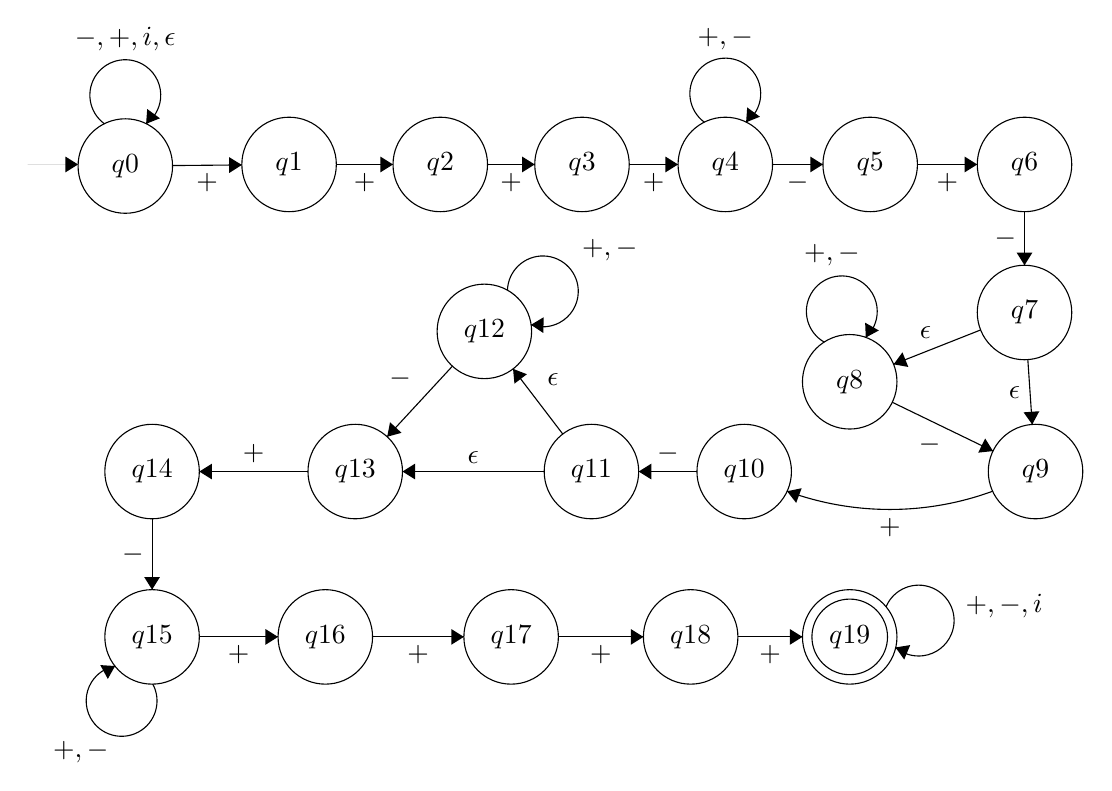
\begin{tikzpicture}[scale=0.2]
\tikzstyle{every node}+=[inner sep=0pt]
\draw [black] (6.2,-11.8) circle (3);
\draw (6.2,-11.8) node {$q0$};
\draw [black] (16.6,-11.7) circle (3);
\draw (16.6,-11.7) node {$q1$};
\draw [black] (26.2,-11.7) circle (3);
\draw (26.2,-11.7) node {$q2$};
\draw [black] (35.2,-11.7) circle (3);
\draw (35.2,-11.7) node {$q3$};
\draw [black] (44.3,-11.7) circle (3);
\draw (44.3,-11.7) node {$q4$};
\draw [black] (53.5,-11.7) circle (3);
\draw (53.5,-11.7) node {$q5$};
\draw [black] (63.3,-11.7) circle (3);
\draw (63.3,-11.7) node {$q6$};
\draw [black] (63.3,-21.1) circle (3);
\draw (63.3,-21.1) node {$q7$};
\draw [black] (52.2,-25.5) circle (3);
\draw (52.2,-25.5) node {$q8$};
\draw [black] (64,-31.2) circle (3);
\draw (64,-31.2) node {$q9$};
\draw [black] (45.5,-31.2) circle (3);
\draw (45.5,-31.2) node {$q10$};
\draw [black] (35.8,-31.2) circle (3);
\draw (35.8,-31.2) node {$q11$};
\draw [black] (29,-22.3) circle (3);
\draw (29,-22.3) node {$q12$};
\draw [black] (20.8,-31.2) circle (3);
\draw (20.8,-31.2) node {$q13$};
\draw [black] (7.9,-31.2) circle (3);
\draw (7.9,-31.2) node {$q14$};
\draw [black] (7.9,-41.7) circle (3);
\draw (7.9,-41.7) node {$q15$};
\draw [black] (18.9,-41.7) circle (3);
\draw (18.9,-41.7) node {$q16$};
\draw [black] (30.7,-41.7) circle (3);
\draw (30.7,-41.7) node {$q17$};
\draw [black] (42.1,-41.7) circle (3);
\draw (42.1,-41.7) node {$q18$};
\draw [black] (52.2,-41.7) circle (3);
\draw (52.2,-41.7) node {$q19$};
\draw [black] (52.2,-41.7) circle (2.4);
\draw [black] (4.877,-9.12) arc (234:-54:2.25);
\draw (6.2,-4.55) node [above] {$-,+,i,\epsilon$};
\fill [black] (7.52,-9.12) -- (8.4,-8.77) -- (7.59,-8.18);
\draw [black] (9.2,-11.77) -- (13.6,-11.73);
\fill [black] (13.6,-11.73) -- (12.8,-11.24) -- (12.8,-12.24);
\draw (11.4,-12.26) node [below] {$+$};
\fill [black] (0,-11.7) -- (2.5,-11.7);
\fill [black] (3.2,-11.7) -- (2.4,-11.2) -- (2.4,-12.2);
\draw [black] (19.6,-11.7) -- (23.2,-11.7);
\fill [black] (23.2,-11.7) -- (22.4,-11.2) -- (22.4,-12.2);
\draw (21.4,-12.2) node [below] {$+$};
\draw [black] (29.2,-11.7) -- (32.2,-11.7);
\fill [black] (32.2,-11.7) -- (31.4,-11.2) -- (31.4,-12.2);
\draw (30.7,-12.2) node [below] {$+$};
\draw [black] (38.2,-11.7) -- (41.3,-11.7);
\fill [black] (41.3,-11.7) -- (40.5,-11.2) -- (40.5,-12.2);
\draw (39.75,-12.2) node [below] {$+$};
\draw [black] (42.977,-9.02) arc (234:-54:2.25);
\draw (44.3,-4.45) node [above] {$+,-$};
\fill [black] (45.62,-9.02) -- (46.5,-8.67) -- (45.69,-8.08);
\draw [black] (47.3,-11.7) -- (50.5,-11.7);
\fill [black] (50.5,-11.7) -- (49.7,-11.2) -- (49.7,-12.2);
\draw (48.9,-12.2) node [below] {$-$};
\draw [black] (56.5,-11.7) -- (60.3,-11.7);
\fill [black] (60.3,-11.7) -- (59.5,-11.2) -- (59.5,-12.2);
\draw (58.4,-12.2) node [below] {$+$};
\draw [black] (63.3,-14.7) -- (63.3,-18.1);
\fill [black] (63.3,-18.1) -- (63.8,-17.3) -- (62.8,-17.3);
\draw (62.8,-16.4) node [left] {$-$};
\draw [black] (63.51,-24.09) -- (63.79,-28.21);
\fill [black] (63.79,-28.21) -- (64.24,-27.37) -- (63.24,-27.44);
\draw (63.05,-26.19) node [left] {$\epsilon$};
\draw [black] (60.51,-22.21) -- (54.99,-24.39);
\fill [black] (54.99,-24.39) -- (55.92,-24.56) -- (55.55,-23.63);
\draw (57.01,-22.79) node [above] {$\epsilon$};
\draw [black] (50.587,-22.984) arc (240.4032:-47.5968:2.25);
\draw (51.07,-18.15) node [above] {$+,-$};
\fill [black] (53.22,-22.69) -- (54.05,-22.24) -- (53.18,-21.75);
\draw [black] (54.9,-26.8) -- (61.3,-29.9);
\fill [black] (61.3,-29.9) -- (60.8,-29.1) -- (60.36,-30);
\draw (57.28,-28.85) node [below] {$-$};
\draw [black] (61.276,-32.45) arc (-69.87784:-110.12216:18.97);
\fill [black] (48.22,-32.45) -- (48.8,-33.19) -- (49.15,-32.26);
\draw (54.75,-34.11) node [below] {$+$};
\draw [black] (42.5,-31.2) -- (38.8,-31.2);
\fill [black] (38.8,-31.2) -- (39.6,-31.7) -- (39.6,-30.7);
\draw (40.65,-30.7) node [above] {$-$};
\draw [black] (33.98,-28.82) -- (30.82,-24.68);
\fill [black] (30.82,-24.68) -- (30.91,-25.62) -- (31.7,-25.02);
\draw (32.97,-25.35) node [right] {$\epsilon$};
\draw [black] (32.8,-31.2) -- (23.8,-31.2);
\fill [black] (23.8,-31.2) -- (24.6,-31.7) -- (24.6,-30.7);
\draw (28.3,-30.7) node [above] {$\epsilon$};
\draw [black] (17.8,-31.2) -- (10.9,-31.2);
\fill [black] (10.9,-31.2) -- (11.7,-31.7) -- (11.7,-30.7);
\draw (14.35,-30.7) node [above] {$+$};
\draw [black] (30.465,-19.696) arc (178.36885:-109.63115:2.25);
\draw (35.17,-17.14) node [right] {$+,-$};
\fill [black] (31.96,-21.88) -- (32.74,-22.4) -- (32.77,-21.4);
\draw [black] (26.97,-24.51) -- (22.83,-28.99);
\fill [black] (22.83,-28.99) -- (23.74,-28.74) -- (23.01,-28.07);
\draw (24.37,-25.29) node [left] {$-$};
\draw [black] (7.9,-34.2) -- (7.9,-38.7);
\fill [black] (7.9,-38.7) -- (8.4,-37.9) -- (7.4,-37.9);
\draw (7.4,-36.45) node [left] {$-$};
\draw [black] (7.941,-44.688) arc (28.51765:-259.48235:2.25);
\draw (3.37,-48.3) node [below] {$+,-$};
\fill [black] (5.55,-43.55) -- (4.61,-43.49) -- (5.09,-44.37);
\draw [black] (10.9,-41.7) -- (15.9,-41.7);
\fill [black] (15.9,-41.7) -- (15.1,-41.2) -- (15.1,-42.2);
\draw (13.4,-42.2) node [below] {$+$};
\draw [black] (21.9,-41.7) -- (27.7,-41.7);
\fill [black] (27.7,-41.7) -- (26.9,-41.2) -- (26.9,-42.2);
\draw (24.8,-42.2) node [below] {$+$};
\draw [black] (33.7,-41.7) -- (39.1,-41.7);
\fill [black] (39.1,-41.7) -- (38.3,-41.2) -- (38.3,-42.2);
\draw (36.4,-42.2) node [below] {$+$};
\draw [black] (45.1,-41.7) -- (49.2,-41.7);
\fill [black] (49.2,-41.7) -- (48.4,-41.2) -- (48.4,-42.2);
\draw (47.15,-42.2) node [below] {$+$};
\draw [black] (54.503,-39.796) arc (157.30497:-130.69503:2.25);
\draw (59.52,-39.73) node [right] {$+,-,i$};
\fill [black] (55.11,-42.37) -- (55.66,-43.14) -- (56.04,-42.22);
\end{tikzpicture}
\end{center}


\section{Definició formal de \nfa{}}

Definim formalment el nostre autòmata. 

\begin{center}
	\dfa $=$ \{Q, $\Sigma{}$*, $\delta$, q0, q19\}
\end{center}

\begin{itemize}
\item \textbf{Q} = \{q0,q1,q2,q3,q4,q5,q6,q7,q8,q9,q10,q11,q12,q13,q14,q15,q16,q17,q18,q19\}
\item $\Sigma$* $=$ \{ + , - , \Return{} , $\epsilon$ \}
\item $\delta$ $=$ Q X $\Sigma$* $\rightarrow$ P(Q) on P(Q) son possibles subconjunts de Q 
\item q0 $\in{}$ Q
\item q19 $\subseteq{}$ Q
\end{itemize}


\subsection{Representació taula $\delta$}

\begin{center}
\begin{table}[ht]
\caption{\label{tab:table-name} $\delta$ table}
\centering
\begin{tabular}{ l l l l l l l l l l l l l l l l l l l l }
\hline
\hline
State & +           & -           & \Return & $\epsilon$              &  &  &  &  &  &  &  &  &  &  &  &  &  &  &  \\ \hline
q0    & \{q0,q1\}   & \{q0\}      & \{q0\}                 & \{q0\}                  &  &  &  &  &  &  &  &  &  &  &  &  &  &  &  \\
q1    & \{q2\}      & $\emptyset$ & $\emptyset$            & $\emptyset$             &  &  &  &  &  &  &  &  &  &  &  &  &  &  &  \\
q2    & \{q3\}      & $\emptyset$ & $\emptyset$            & $\emptyset$             &  &  &  &  &  &  &  &  &  &  &  &  &  &  &  \\
q3    & \{q4\}      & $\emptyset$ & $\emptyset$            & $\emptyset$             &  &  &  &  &  &  &  &  &  &  &  &  &  &  &  \\
q4    & \{q4\}      & \{q4,q5\}   & $\emptyset$            & $\emptyset$             &  &  &  &  &  &  &  &  &  &  &  &  &  &  &  \\
q5    & \{q6\}      & $\emptyset$ & $\emptyset$            & $\emptyset$             &  &  &  &  &  &  &  &  &  &  &  &  &  &  &  \\
q6    & $\emptyset$ & \{q7\}      & $\emptyset$            & $\emptyset$             &  &  &  &  &  &  &  &  &  &  &  &  &  &  &  \\
q7    & $\emptyset$ & $\emptyset$ & $\emptyset$            & \{q8,q9\}               &  &  &  &  &  &  &  &  &  &  &  &  &  &  &  \\
q8    & \{q8\}      & \{q8,q9\}   & $\emptyset$            & $\emptyset$             &  &  &  &  &  &  &  &  &  &  &  &  &  &  &  \\
q9    & \{q10\}     & $\emptyset$ & $\emptyset$            & $\emptyset$             &  &  &  &  &  &  &  &  &  &  &  &  &  &  &  \\
q10   & $\emptyset$ & \{q11\}     & $\emptyset$            & $\emptyset$             &  &  &  &  &  &  &  &  &  &  &  &  &  &  &  \\
q11   & $\emptyset$ & $\emptyset$ & $\emptyset$            & \{q12,q13\}             &  &  &  &  &  &  &  &  &  &  &  &  &  &  &  \\
q12   & \{q12\}     & \{q12,q13\} & $\emptyset$            & $\emptyset$             &  &  &  &  &  &  &  &  &  &  &  &  &  &  &  \\
q13   & \{q14\}     & $\emptyset$ & $\emptyset$            & $\emptyset$             &  &  &  &  &  &  &  &  &  &  &  &  &  &  &  \\
q14   & $\emptyset$ & \{q15\}     & $\emptyset$            & $\emptyset$             &  &  &  &  &  &  &  &  &  &  &  &  &  &  &  \\
q15   & \{q15,q16\} & \{q15\}     & $\emptyset$            & $\emptyset$             &  &  &  &  &  &  &  &  &  &  &  &  &  &  &  \\
q16   & \{q17\}     & $\emptyset$ & $\emptyset$            & $\emptyset$             &  &  &  &  &  &  &  &  &  &  &  &  &  &  &  \\
q17   & \{q18\}     & $\emptyset$ & $\emptyset$            & $\emptyset$             &  &  &  &  &  &  &  &  &  &  &  &  &  &  &  \\
q18   & \{q19\}     & $\emptyset$ & $\emptyset$            & $\emptyset$             &  &  &  &  &  &  &  &  &  &  &  &  &  &  &  \\
q19   & \{q19\}     & \{q19\}     & \{q19\}                & $\emptyset$ &  &  &  &  &  &  &  &  &  &  &  &  &  &  & \\ \hline

\end{tabular}
\end{table}

\end{center}

\clearpage











































\chapter{Push-Down Automata}

\chapter{Turing Machine}



\begin{multicols}{2}
\end{multicols}



\begin{thebibliography}{9}
\bibitem{FC} 
Fundamental of Computation - Michael Sipser
 
\bibitem{patterns}
\hyperlink{http://ima.udg.edu/~rigau/FC/FC_patterns.pdf}{Problema Patterns (i.e., Cerca de Patrons) - Jaume Rigau} 

\bibitem{Hopcroft}
\hyperlink{http://ima.udg.edu/~rigau/FC/MFAP.pdf}{Lexical analisys - part 4}

\bibitem{Manual UTM}
\hyperlink{http://ima.udg.edu/~rigau/FC/utm_read_me.pdf}{Universal Turing Machine - Manual}

\end{thebibliography}

\printindex
\end{document}


